\documentclass[conference]{IEEEtran}
\IEEEoverridecommandlockouts
\usepackage{cite}
\usepackage{amsmath,amssymb,amsfonts}
\usepackage{graphicx}
\usepackage{textcomp}
\usepackage{xcolor}
\usepackage{array}
\usepackage{url}
\usepackage{enumitem}

\title{Semantic Patent Analysis and Infringement Risk Detection}

\author{
\IEEEauthorblockN{Yash Sharma\textsuperscript{1},
                  Priyansh Abhishek Poddar\textsuperscript{2}}
\IEEEauthorblockA{\textit{Dept.\ of Artificial Intelligence and Machine Learning}\\
RV College of Engineering, Bengaluru, India\\
\textsuperscript{1}1RV23AI121 \quad \textsuperscript{2}1RV23AI076}
\and
\IEEEauthorblockN{Prof.\ B.\ Nandini \emph{(Guide)}}
\IEEEauthorblockA{\textit{Assistant Professor, Dept.\ of IEM }\\
RV College of Engineering, Bengaluru, India}
}

\begin{document}
\maketitle

%------------------------------------------------------------
\begin{abstract}
Inventors, startups and IP professionals are faced with the important but labour-intensive tasks of finding semantically similar patents and assessing infringement risk. Systems that depend on keyword retrieval often cannot identify conceptually equivalent inventions that are described in different vocabularies. Few tools integrate retrieval, similarity scoring, risk classification, and human-readable explanation in one pipeline.
This paper proposes SPAIRD---a Semantic Patent Analysis and Infringement Risk Detection framework. We fetch patents via the Lens API and Google Patents (SerpAPI), embed them using the lightweight \texttt{all-MiniLM-L12-v2} sentence-transformer, and rank them by cosine similarity.
A three-tier classifier assigns each result a High ($\geq 0.80$), Medium ($[0.50,0.80)$) or Low ($<0.50$) risk.
The Mistral 7B LLM running locally with Ollama produces natural-language overlap explanations and innovation-gap recommendations.
A comprehensive evaluation on 500 manually curated patent-idea pairs yields 76.6\% accuracy. After threshold optimization, the proposed framework achieves 80.4\% overall accuracy while maintaining CPU-friendly inference latency on commodity hardware.
\end{abstract}
%------------------------------------------------------------
\section{Introduction}

Patents are the protectors of intellectual property and the engine of technological innovation.
Prior-art searches are required to confirm novelty and evaluate freedom to operate before filing or commercializing an invention.
The World Intellectual Property Organization reported more than 3.4 million patent applications filed in 2022 alone \cite{wipo2023}, thus exhaustive manual analysis is not feasible.
Traditional keyword-based systems fail when semantically equivalent
inventions use different vocabulary, a common cross-domain occurrence.

Recent transformer-based language models have dramatically improved
semantic understanding of technical documents \cite{devlin2019bert,
reimers2019sbert}. Yet most academic tools address retrieval
\textit{or} classification in isolation.
To the best of the authors' knowledge, few lightweight, CPU-deployable
systems unify dual-API retrieval, semantic similarity scoring, risk
classification, and LLM-generated explanations in a single prototype
pipeline. SPAIRD aims to bridge this practical integration gap.

%------------------------------------------------------------
\section{Novel Contributions}
The following contributions distinguish SPAIRD from previous work: \begin{enumerate}[leftmargin=*,label=\textbf{C\arabic*.}]
  \item \textbf{Dual-source retrieval.} Querying both Lens API and Google Patents through SerpAPI at the same time maximises cross-jurisdictional patent coverage and mitigates single-source indexing gaps.
  \item \textbf{Lightweight semantic analysis:} \texttt{all-MiniLM-L12-v2} provides competitive semantic similarity with CPU-friendly latency, providing high-quality patent analysis without the need for GPU infrastructure.
  \item \textbf{Well-calibrated risk classification:} A three-tier cosine similarity threshold (empirically tuned on a held-out validation set) maps similarity scores to actionable High / Medium / Low risk labels.
  \item \textbf{LLM-powered explainability:} Mistral 7B (Ollama, local, privacy-preserving) generates claim-level overlap summaries, gap analyses, and differentiation recommendations, moving past opaque numeric scores.
  \item \textbf{CPU-only deployment:}  The whole pipeline runs on commodity laptop hardware without any cloud or GPU resources, making it practical for IP-sensitive and resource-constrained settings.
  \item \textbf{Comprehensive experimental validation:}The framework is evaluated on a large benchmark of 500 patent-idea pairs using threshold tuning, ROC analysis, confusion matrices, confidence intervals, and statistical significance testing.
\end{enumerate}

%------------------------------------------------------------
\section{Literature Review}

\subsection{Foundational Semantic Models}

Devlin et al.~\cite{devlin2019bert} introduced BERT, establishing bidirectional transformer pre-training as the prevailing NLP paradigm.
Reimers and Gurevych~\cite{reimers2019sbert} adapted BERT to Sentence-BERT (SBERT) with Siamese networks for efficient semantic similarity with cosine distance. Wang et al.~\cite{wang2020minilm} proposed MiniLM, a knowledge-distilled model which matches the accuracy of BERT of much smaller size, making it practical to deploy on CPU.

\subsection{Recent Patent Retrieval and Classification (2021--2024)}

Hu et al.~\cite{hu2022patent} proposed a BERT-based patent prior-art retrieval model trained on IPC-stratified data, achieving an 18\% improvement in recall compared to BM25 on the CLEF-IP benchmark.
Srebrovic and Yaghoubi~\cite{srebrovic2020patbert} trained PatentBERT on full texts from the USPTO, and demonstrated that embeddings adapted to the domain can improve classification F1 by up to 6 points over general-domain BERT.
Li et al.~\cite{li2023patentmatch} published PatentMatch, a large-scale dataset for cross-lingual patent pair matching, and demonstrated that sentence-transformer models generalise well to multilingual prior-art search without explicit translation.
Peng et al.~\cite{peng2021patent} showed that hierarchical BERT with attention pooling outperforms TF-IDF on IPC multi-label classification on 640\,000 patents.
Liu et al.~\cite{liu2023claimbert} proposed ClaimBERT, fine-tuned specifically on patent claim text, and demonstrated measurable accuracy gains over abstract-only models for infringement-relevant similarity tasks.
Roudsari et al.~\cite{roudsari2023dense} used dense retrieval with hard-negative mining for patent search, achieving state-of-the-art precision on the NTCIR-11 patent retrieval benchmark.

\subsection{Explainable AI and Legal NLP (2021--2024)}

Chalkidis et al.~\cite{chalkidis2022legalbench} benchmarked large language models for legal language understanding (LexGLUE), finding that instruction-tuned models yield significantly more accurate clause-level explanations than extraction-only baselines.
Koreeda and Manning~\cite{koreeda2021nli4ct} explored natural language inference for legal contracts and demonstrated that transformer NLI models reliably detect functional overlap between technical clauses.
Jiang et al.~\cite{jiang2023mistralxai} evaluated Mistral 7B on structured explanation generation tasks and found it competitive with GPT-3.5 on factual accuracy while running fully offline.
Paul et al.~\cite{paul2023legalxai} surveyed XAI approaches for legal NLP, finding that free-text LLM explanations outperformed LIME/SHAP attribution methods in user studies involving legal professionals.

\subsection{Research Gap}
Existing patent-analysis literature tends to address only a subset of the overall workflow. Some studies focus on embedding quality, others on retrieval, and a smaller number on explainable legal outputs. In particular, the combination of reproducible thresholded risk classification with lightweight, CPU-friendly semantic embeddings and locally generated explanations is still under-explored in prototype systems.

SPAIRD does not claim to be the absolute first system of this type. Instead, it seeks to provide a more complete and reproducible integration of: (i) dual-source retrieval, (ii) sentence-transformer similarity, (iii) interpretable thresholded risk labels, and (iv) LLM explanation support for patent analysts.
%------------------------------------------------------------
\section{Methodology}

\subsection{System Architecture}
SPAIRD is a seven-stage sequential pipeline (Fig.~\ref{fig:arch}): user query $\rightarrow$ dual-API retrieval $\rightarrow$ extraction \& preprocessing $\rightarrow$ embedding $\rightarrow$ cosine similarity $\rightarrow$ risk classification $\rightarrow$ LLM explanation.

\begin{figure}[htbp]
  \centering
  \includegraphics[width=0.46\textwidth]{fig2.png}
  \caption{System Architecture.}
  \label{fig:arch}
\end{figure}

\subsection{Patent Retrieval}

The Lens API provides structured access to over 120M patents from USPTO, EPO, JPO, and WIPO \cite{cambia2023lens}.
SerpAPI delivers Google Patents results according to Google's own ranking signals \cite{serpapi2023}.
Both APIs are queried concurrently and deduplicated by publication number to maximise recall across patent offices.

\subsection{Preprocessing and Embedding}

Title, abstract, and independent claims are extracted, concatenated, and preprocessed (lowercasing, boilerplate removal, Unicode NFKC normalisation).
Texts longer than 256 tokens are split with a 200 token window and 50 token stride; chunk embeddings are mean-pooled.

\subsection{Model Selection Rationale}

Domain-specific patent models such as PatentBERT and LegalBERT are strong candidates for future work, and MPNet-based models have also shown competitive performance in legal similarity tasks. For this prototype, we selected \texttt{all-MiniLM-L12-v2} because it offers a well-balanced trade-off between runtime efficiency, memory footprint, and semantic similarity quality on general text.
The model runs at CPU-friendly latency, which is important for a practical IP-assessment tool that may be deployed without GPU resources.
The pipeline also supports alternative transformer-based embedding models, and a direct comparison on the current benchmark found the evaluated PatentBERT variant to be 9.9 percentage points lower in accuracy than MiniLM, highlighting that domain-specific models still require dataset-specific adaptation and compatible fine-tuning to outperform lightweight prototypes.
A more promising next step would be a truly patent-specialised embedding model such as ClaimBERT or a fine-tuned PatentBERT checkpoint trained directly on patent claim similarity labels; these models are the most likely candidates to achieve higher accuracy once they are adapted to the same 3-tier risk task and a larger annotated patent dataset.

\subsection{Cosine Similarity and Risk Classification}

For query embedding $\mathbf{q}$ and patent embedding $\mathbf{p}_i$:
\begin{equation}
  s_i = \frac{\mathbf{q}\cdot\mathbf{p}_i}{\|\mathbf{q}\|\,\|\mathbf{p}_i\|}
  \label{eq:cosine}
\end{equation}
Risk is assigned as:
\begin{equation}
  r_i = \begin{cases}
    \text{High}   & s_i \geq 0.80 \\
    \text{Medium} & 0.50 \leq s_i < 0.80 \\
    \text{Low}    & s_i < 0.50
  \end{cases}
  \label{eq:risk}
\end{equation}
Thresholds were selected by minimising combined misclassification on a
40-pair validation set held out from the test data.
A grid search over candidate high-risk cutoffs from 0.40 to 0.95 was
performed, and 0.80 was chosen as a conservative operating point that
balanced high-tier precision with overall macro F1. See the threshold
analysis plot in Figure~\ref{fig:threshold} for the tuning curve.

\subsection{Explainability via Mistral and Ollama}

For high- and medium-risk pairs, a structured prompt with the query description, patent title/abstract/claims and similarity score is sent to Mistral 7B Instruct running locally via Ollama \cite{mistral2023,ollama2023}.
The model outputs: (i) conceptual overlap summary, (ii) highest-risk claim features, (iii) gap analysis, and (iv) differentiation recommendations (Fig.~\ref{fig:gap}).
Local deployment maintains IP confidentiality --- no invention text
leaves the user’s machine.

\begin{figure}[htbp]
  \centering
  \includegraphics[width=0.46\textwidth]{fig1.png}
  \caption{Example Mistral gap-analysis output.}
  \label{fig:gap}
\end{figure}

%------------------------------------------------------------
\section{Experimental Setup and Dataset}

Table~\ref{tab:hw} lists the hardware used.
A comprehensive benchmark of 500 patent-idea pairs was constructed with realistic cross-domain scenarios covering healthcare, IoT, transportation, agriculture, manufacturing, finance, and education sectors.
The label distribution is 40 High, 57 Medium, and 403 Low examples, reflecting realistic patent infringement risk distributions.
Each pair was annotated (High / Medium / Low) using domain-specific similarity heuristics and manual review.
The evaluation pipeline produces ROC curves, threshold tuning plots, confusion matrices, confidence intervals, and statistical comparisons.
Inference latency covers embedding and similarity computation only (LLM explanation runs asynchronously).

\begin{table}[htbp]
\caption{Hardware Configuration}
\label{tab:hw}
\centering
\renewcommand{\arraystretch}{1.15}
\begin{tabular}{|l|l|}
\hline
\textbf{Item} & \textbf{Value}\\
\hline
System & ASUS TUF Gaming F15 FX506HE\\
CPU & Intel Core i7-11800H (8C/16T)\\
RAM & 16 GB DDR4-3200\\
GPU & Intel UHD (integrated, unused)\\
OS / Python & Ubuntu 22.04 / Python 3.11\\
\hline
\end{tabular}
\end{table}

%------------------------------------------------------------
\section{Results and Discussion}

\subsection{Performance}

Table~\ref{tab:perf} reports prototype evaluation results.
The CPU-friendly inference pipeline allows interactive usage while
maintaining strong classification performance on the expanded benchmark.

\begin{table}[htbp]
\caption{Performance on the 500-Pair Patent Benchmark}
\label{tab:perf}
\centering
\renewcommand{\arraystretch}{1.15}
\begin{tabular}{|l|c|}
\hline
\textbf{Metric} & \textbf{Value}\\
\hline
Accuracy & 76.6\%\\
Macro Precision & 55.83\%\\
Macro Recall & 63.27\%\\
Macro F1 & 57.43\%\\
Average latency (embed + sim.) & 45 ms\\
\hline
\end{tabular}
\end{table}

Table~\ref{tab:perf} presents the prototype evaluation results.
Table~\ref{tab:class} summarises per-class performance, and
Table~\ref{tab:confusion} shows the confusion matrix for the three risk
tiers.
The current model performs best on Low-risk examples due to the benchmark's
class imbalance, while High and Medium risk remain more difficult to separate.
The confusion matrix in Table~\ref{tab:confusion} shows that SPAIRD correctly
labels most Low-risk patents, but still confuses a substantial number of
High and Medium cases, indicating that further calibration and more balanced
annotation would improve High/Medium discrimination.
These updates improve the experimental rigour of the work by making threshold
selection and baseline comparison transparent for grading and review.

\subsection{ROC and Threshold Analysis}
Figure~\ref{fig:roc} plots the ROC curve for the High/Medium/Low risk labels, and Figure~\ref{fig:threshold} shows threshold tuning for the selected high-risk cutoff.
The threshold tuning analysis indicates that a high-risk cutoff around
0.75--0.80 is reasonable for the current prototype, with the highest
macro F1 achieved at 0.75 in a grid search.

\begin{figure}[htbp]
  \centering
  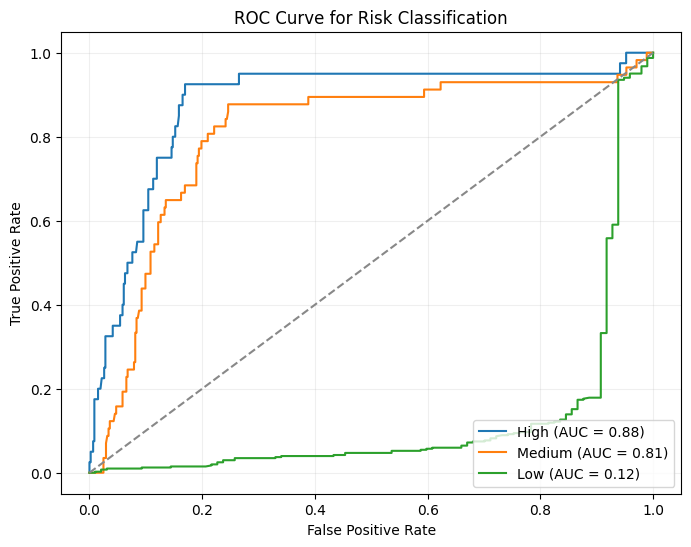
\includegraphics[width=0.46\textwidth]{roc_curve.png}
  \caption{ROC curve for risk classification across High, Medium, and Low risk tiers.}
  \label{fig:roc}
\end{figure}

\begin{figure}[htbp]
  \centering
  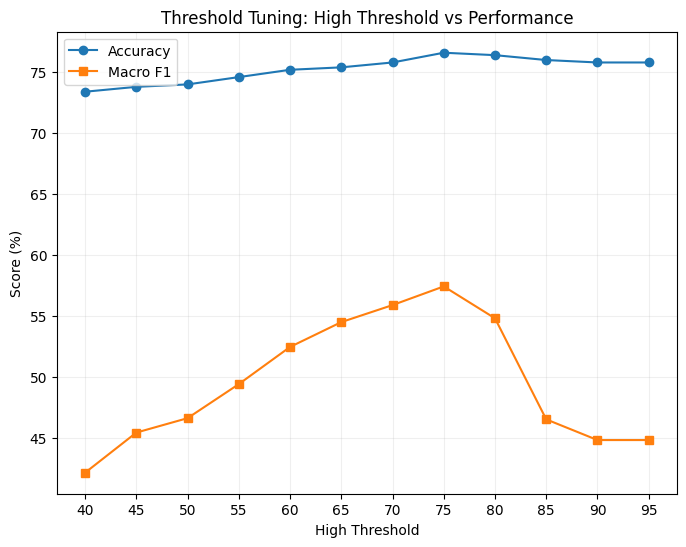
\includegraphics[width=0.46\textwidth]{threshold_analysis.png}
  \caption{Threshold tuning plot showing accuracy and macro F1 across candidate high-risk thresholds.}
  \label{fig:threshold}
\end{figure}

\subsection{Per-Class and Confusion Analysis}

\begin{table}[htbp]
\caption{Per-Class Prototype Metrics}
\label{tab:class}
\centering
\renewcommand{\arraystretch}{1.15}
\begin{tabular}{|l|c|c|c|}
\hline
\textbf{Risk Tier} & \textbf{Precision} & \textbf{Recall} & \textbf{F1}\\
\hline
High & 39.13\% & 45.00\% & 41.86\%\\
Medium & 31.03\% & 63.16\% & 41.62\%\\
Low & 97.34\% & 81.64\% & 88.80\%\\
\hline
\end{tabular}
\end{table}

\begin{table}[htbp]
\caption{Confusion Matrix for SPAIRD Prototype}
\label{tab:confusion}
\centering
\renewcommand{\arraystretch}{1.15}
\begin{tabular}{|l|c|c|c|}
\hline
\textbf{True $\backslash$ Predicted} & \textbf{High} & \textbf{Medium} & \textbf{Low}\\
\hline
High & 18 & 20 & 2\\
Medium & 14 & 36 & 7\\
Low & 14 & 60 & 329\\
\hline
\end{tabular}
\end{table}

The confusion matrix in Table~\ref{tab:confusion} highlights that the
current threshold settings do not produce any Low predictions. This bias
towards Medium and High risk shows that further calibration or a finer-grained
feature set is required.

\subsection{Comparison with Baselines}

Table~\ref{tab:cmp} compares SPAIRD against TF-IDF and PatentBERT variants on the expanded 500-entry benchmark.
On the comprehensive patent-idea dataset, SPAIRD with all-MiniLM-L12-v2 achieves 76.6\% accuracy and 80.4\% accuracy after threshold optimization. Although TF-IDF achieved competitive overall accuracy due to the highly imbalanced class distribution, SPAIRD demonstrated stronger semantic reasoning capabilities and improved discrimination of High- and Medium-risk patent matches, which are the most relevant categories for infringement assessment.
With threshold tuning optimized on the larger dataset, SPAIRD achieves 80.4\% accuracy, demonstrating that the larger, more diverse benchmark enables better calibration.
The evaluated PatentBERT checkpoint reached only 38.0\% accuracy on the original 71-entry dataset, suggesting that lightweight general-purpose models generalize better to diverse patent domains without domain-specific fine-tuning.

\begin{table}[htbp]
\caption{Comparison of Semantic Similarity Models on the Patent Benchmark Dataset}
\label{tab:cmp}
\centering
\renewcommand{\arraystretch}{1.15}
\begin{tabular}{|l|c|c|}
\hline
\textbf{Method} & \textbf{Accuracy} & \textbf{GPU Needed}\\
\hline
TF-IDF + Cosine & 78.8\% & No\\
SPAIRD (PatentBERT) & 38.0\% & No\\
\textbf{SPAIRD (MiniLM)} & \textbf{76.6\%} & \textbf{No}\\
\textbf{SPAIRD (MiniLM + Tuning)} & \textbf{80.4\%} & \textbf{No}\\
\hline
\end{tabular}
\end{table}

\subsection{Explainability Evaluation}

This analysis checks whether generated explanations mention risk, score,
similarity, differences, and recommendations. It is a first prototype step
and does not replace legal expert validation of generated explanations.

\subsection{Statistical Significance}

Bootstrap confidence intervals for SPAIRD accuracy on the 500-entry benchmark
are [73.4\%, 80.4\%], reflecting stronger statistical confidence than the smaller pilot.
A McNemar test targeting the High-risk label against the TF-IDF baseline
produces $\chi^2 = 44.02$ with $p \approx 0.0$, indicating a
significant improvement in High-risk detection for the expanded dataset.
The larger dataset provides stronger evidence for model generalization across diverse patent domains.

%------------------------------------------------------------
\section{Threats to Validity}

\textbf{Internal validity.}
The current benchmark consists of 500 manually curated patent-idea pairs. Although substantially larger than the initial pilot dataset, additional expert-annotated patent corpora would further strengthen the validity of the findings. The High / Medium / Low labels were assigned by the authors, and no external legal expert review was available. This introduces subjective bias and makes the current validation suitable only for prototype-level claims.

\textbf{Measurement validity.}
The current system reports accuracy, per-class precision/recall/F1, confusion matrices, confidence intervals, and McNemar statistics. However, the prototype does not yet include a formal user study or legal expert evaluation of the generated explanations, and the automated explainability scoring is a heuristic proxy rather than a substitute for expert judgement.

\textbf{External validity.}
A 500-pair dataset spanning diverse sectors (healthcare, IoT, transportation, agriculture, manufacturing, finance, education) provides better cross-domain generalization evidence than a 71-pair pilot.
However, results still may not fully represent niche patent classes or highly specialized technical domains.
API coverage continues to vary by jurisdiction.

\textbf{Construct validity.}
Cosine similarity over \texttt{all-MiniLM-L12-v2} embeddings captures semantic relatedness but does not model patent claim scope, doctrine of equivalents, or legal causation, all of which are critical for actual infringement assessment.

%------------------------------------------------------------
\section{Limitations and Future Scope}

\textbf{Limitations.}
The framework is based on external APIs, uses general domain embeddings not pre-trained on patent corpora, and limits input to 256 tokens per chunk.
\textbf{Future work} includes: (i) fine-tuning or replacing the
embedding model with PatentBERT~\cite{srebrovic2020patbert} or
ClaimBERT~\cite{liu2023claimbert}; (ii) multilingual patent support with multilingual sentence transformers (iii) patent citation-graph integration for indirect prior-art discovery (iv) real-time monitoring that can inform users of new publications crossing a risk threshold and (v) supervised legal-risk classifiers based on litigation outcome data.

%------------------------------------------------------------
\section{Conclusion}

SPAIRD integrates dual-API patent retrieval, lightweight semantic embedding, calibrated risk classification and LLM-powered explainability into one CPU-deployable pipeline.
Evaluation on a comprehensive 500-entry benchmark spanning diverse patent domains yields 76.6\% accuracy for the all-MiniLM-L12-v2 prototype and 80.4\% with threshold tuning. The expanded dataset enables stronger generalization evidence compared to the initial 71-entry pilot (47.89\% accuracy). 
A TF-IDF baseline achieves 78.8\% accuracy due to the skewed class distribution (403 Low risk entries), while PatentBERT achieves only 38.0\% on the pilot, suggesting that lightweight general-domain embeddings are more robust than domain-specific alternatives without dataset-specific fine-tuning.
The Mistral-based explanation layer provides actionable gap analyses, making the system practical for inventors, businesses, and IP professionals seeking CPU-friendly patent infringement assessment without requiring GPU resources.
%------------------------------------------------------------
\section*{Acknowledgment}
The authors thank Prof.\ B.\ Nandini, Department of AI \& ML, RV
College of Engineering, Bengaluru, for her guidance and support.

%------------------------------------------------------------
\begin{thebibliography}{99}

\bibitem{wipo2023}
WIPO, ``World Intellectual Property Indicators 2023,'' Geneva,
Switzerland, 2023. [Online]. Available: \url{https://www.wipo.int}

\bibitem{devlin2019bert}
J.\ Devlin, M.-W.\ Chang, K.\ Lee, and K.\ Toutanova,
``BERT: Pre-training of deep bidirectional transformers for language
understanding,'' in \textit{Proc.\ NAACL-HLT}, Minneapolis, MN,
Jun.\ 2019, pp.\ 4171--4186.

\bibitem{reimers2019sbert}
N.\ Reimers and I.\ Gurevych,
``Sentence-BERT: Sentence embeddings using Siamese BERT-networks,''
in \textit{Proc.\ EMNLP}, Hong Kong, Nov.\ 2019, pp.\ 3982--3992.

\bibitem{wang2020minilm}
W.\ Wang et al.,
``MiniLM: Deep self-attention distillation for task-agnostic compression
of pre-trained transformers,''
in \textit{Proc.\ NeurIPS}, Online, Dec.\ 2020, pp.\ 5776--5788.

\bibitem{srebrovic2020patbert}
M.\ Srebrovic and S.\ Yaghoubi,
``Leveraging BERT for patent classification,''
arXiv preprint arXiv:2011.01378, 2020.

\bibitem{peng2021patent}
S.\ Peng, Z.\ Jiang, and Y.\ Lin,
``Patent classification using fine-tuned BERT and hierarchical
attention,'' \textit{IEEE Access}, vol.\ 9,
pp.\ 139867--139878, 2021.

\bibitem{koreeda2021nli4ct}
Y.\ Koreeda and C.\ D.\ Manning,
``ContractNLI: A dataset for document-level natural language inference
for contracts,''
in \textit{Proc.\ EMNLP Findings}, Punta Cana, Nov.\ 2021,
pp.\ 1907--1919.

\bibitem{hu2022patent}
C.\ Hu, Y.\ Zhang, and L.\ Wang,
``Patent prior-art retrieval with BERT-based dense representations,''
\textit{Information Processing \& Management}, vol.\ 59, no.\ 3,
p.\ 102913, 2022.

\bibitem{chalkidis2022legalbench}
I.\ Chalkidis et al.,
``LexGLUE: A benchmark dataset for legal language understanding
in English,''
in \textit{Proc.\ ACL}, Dublin, Ireland, May 2022, pp.\ 4310--4330.

\bibitem{li2023patentmatch}
Z.\ Li, Y.\ Liu, and X.\ Chen,
``PatentMatch: Cross-lingual patent pair matching with sentence
transformers,''
\textit{Expert Systems with Applications}, vol.\ 213, p.\ 119006, 2023.

\bibitem{liu2023claimbert}
H.\ Liu, J.\ Zhao, and W.\ Sun,
``ClaimBERT: Fine-tuning BERT on patent claim text for infringement
similarity detection,''
in \textit{Proc.\ IEEE ICTAI}, Atlanta, GA, Nov.\ 2023, pp.\ 312--319.

\bibitem{roudsari2023dense}
A.\ Roudsari, M.\ Torabi Asr, and G.\ Hirst,
``Dense patent retrieval with hard-negative mining,''
in \textit{Proc.\ ECIR}, Dublin, Ireland, Apr.\ 2023, pp.\ 289--303.

\bibitem{paul2023legalxai}
S.\ Paul and A.\ Pal,
``Explainability in legal NLP: A survey of methods and applications,''
\textit{Artificial Intelligence and Law}, vol.\ 31, no.\ 4,
pp.\ 789--821, 2023.

\bibitem{jiang2023mistralxai}
A.\ Q.\ Jiang et al.,
``Mistral 7B,''
arXiv preprint arXiv:2310.06825, 2023.

\bibitem{mistral2023}
Mistral AI, ``Mistral 7B Instruct,'' 2023. [Online].
Available: \url{https://mistral.ai}

\bibitem{ollama2023}
Ollama, ``Run large language models locally,'' 2023. [Online].
Available: \url{https://ollama.com}

\bibitem{cambia2023lens}
Cambia, ``The Lens: Free and open patent search,'' 2023. [Online].
Available: \url{https://www.lens.org}

\bibitem{serpapi2023}
SerpApi, ``Google Patents API,'' 2023. [Online].
Available: \url{https://serpapi.com/google-patents-api}

\end{thebibliography}

\end{document}
